\documentclass[main.tex]{subfiles}
\begin{document}
\section{Implementation}
All code is available on GitHub \href{https://github.com/DNedilko/CausalDiscoveryProject/tree/244b50fed45bf1547cf7d0a1053891f276ac663b/Project}{DNedilko/CausalDiscovery}. The main language of implementation is Python. 
\subsection{Causal Discovery Setup}
Causal Discovery implementation is in the \href{https://github.com/DNedilko/CausalDiscoveryProject/blob/main/Project/fci_runner.py}{fci\_runner.py} on GitHub. 
The workflow of the Python code begins with data preparation. The \textt{data\_loader} function ingests a specified subset of columns from a large dataset (HBSC) and has the option to stratify by sex. This data is then cleaned using the \textt{data\_prep} function, which removes rows with missing values according to the specifications outlined in Data Section and converts the data into a numeric format suitable for subsequent analysis. Textual categorical values are label-encoded, and the DataFrame is transformed into a NumPy array. This ensures that the resulting matrix meets the requirements of the libraries being used.

After data preparation, the pipeline executes the FCI algorithm. The \textt{run\_fci} function applies FCI from \texttt{causal-inference} package to the cleaned data, utilising $G^2$ and $\chi^2$ as the conditional independence test at a specified significance level. The output is a Partial Ancestral Graph (PAG) that encodes the inferred causal relationships among variables. This graph is then visualised and saved as a PNG image. To facilitate a comprehensive analysis, the \texttt{iterator\_over\_fci} function performs parallel execution of FCI across multiple conditional independence tests and significance levels.

 The used \texttt{causal-learn} library follows the algorithm in the Methodology. Besides that, it allows for background knowledge. This function enables the restriction of testing sets during the adjacency identification step of FCI\cite{causal-learn-docs}. 
 Example of use is available in the Appendix \ref{appendix: python_fci_clean}.

\subsection{Parameter Choices}

The conditional independence (CI) tests $G^2$ and $\chi^2$ are asymptotically similar. To assess which test would perform better in terms of runtime, we experimented by comparing their scalability. We found that, for the given dataset, the $\chi^2$ test scaled less efficiently. This may be since the $G^2$ test handles zero counts more robustly and relies on logarithmic operations (see Figure~\ref{fig:fci_runtime_vs_samplesize}).

Furthermore, $G^2$ is more stable under changes in the significance level $\alpha$, and its runtime does not increase as sharply compared to the $\chi^2$ test(see Figure~\ref{fig:fci_runtime_vs_alpha}). Based on these findings, we chose the $G^2$ test for all subsequent experiments.
\begin{figure}[h]
    \centering
    \begin{minipage}{0.48\textwidth}
        \centering
        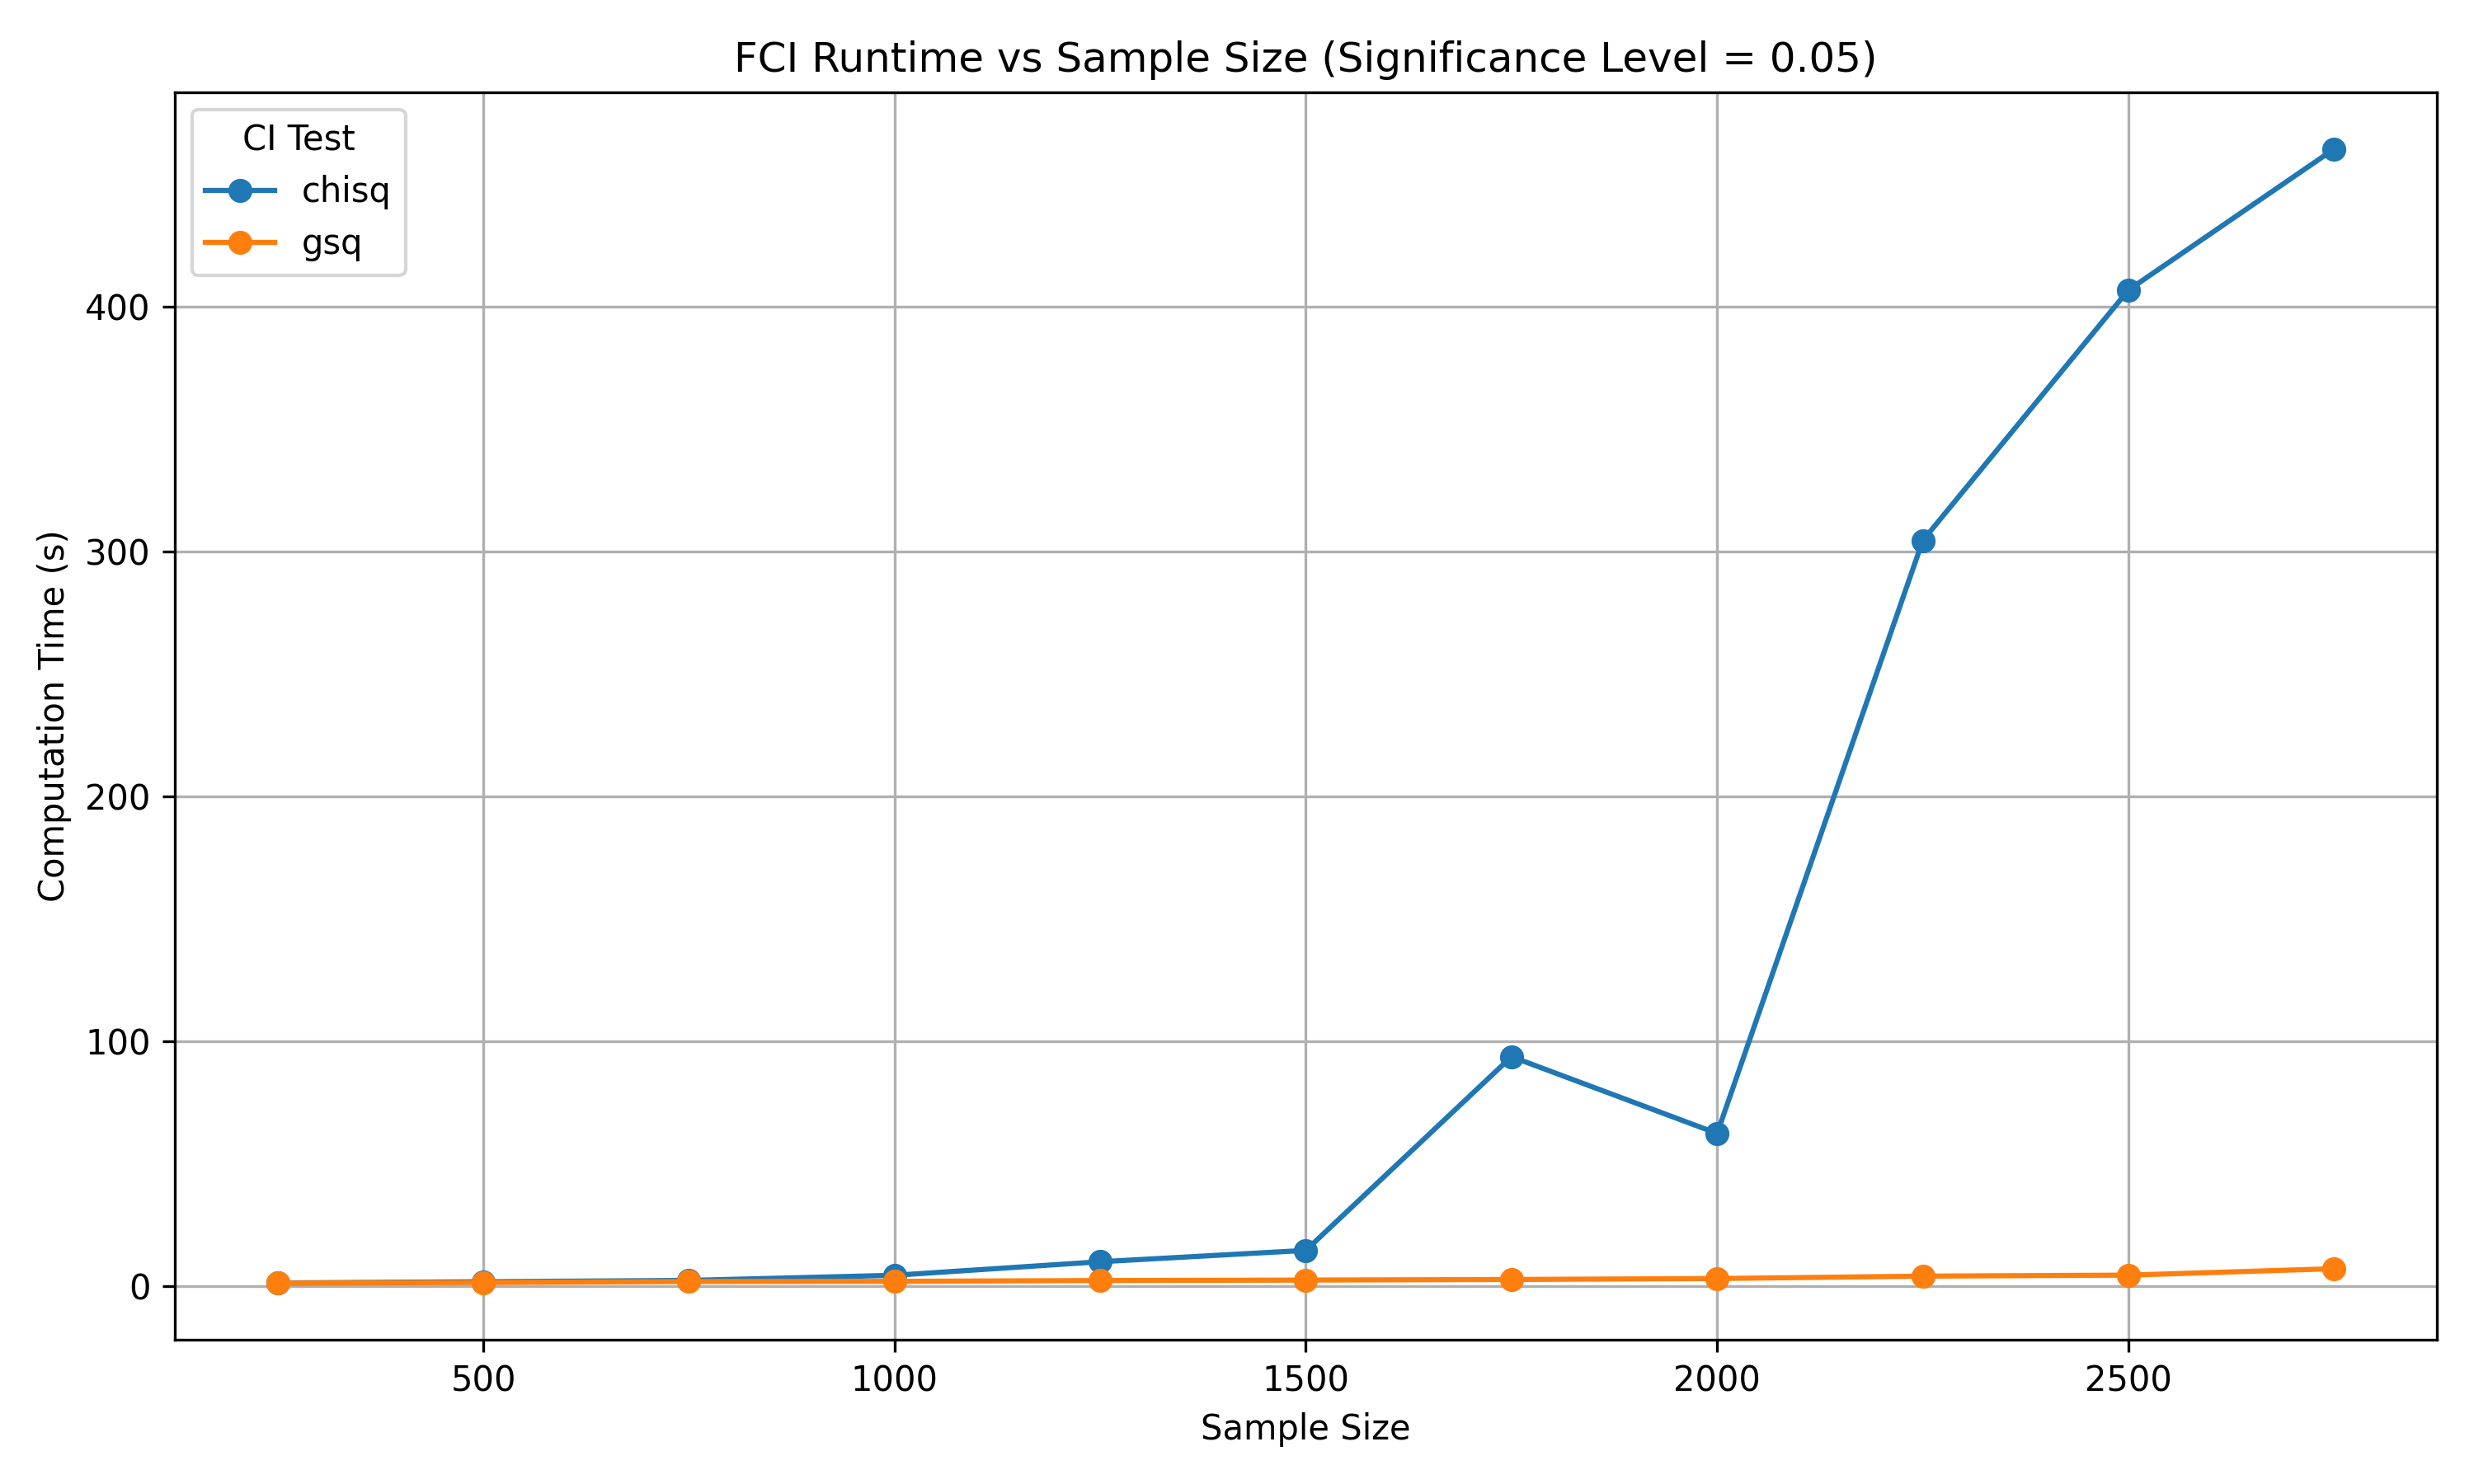
\includegraphics[width = 1\linewidth]{Report/final_report/pictures/fci_runtime_vs_samplesize.png}
        \caption{Computation time of the FCI algorithm as a function of sample size for different CI tests. The significance level $\alpha$ is fixed at 0.05 to isolate the effect of increasing data volume on performance.}
        \label{fig:fci_runtime_vs_samplesize}
    \end{minipage}\hfill
    \begin{minipage}{0.48\textwidth}
        \centering
        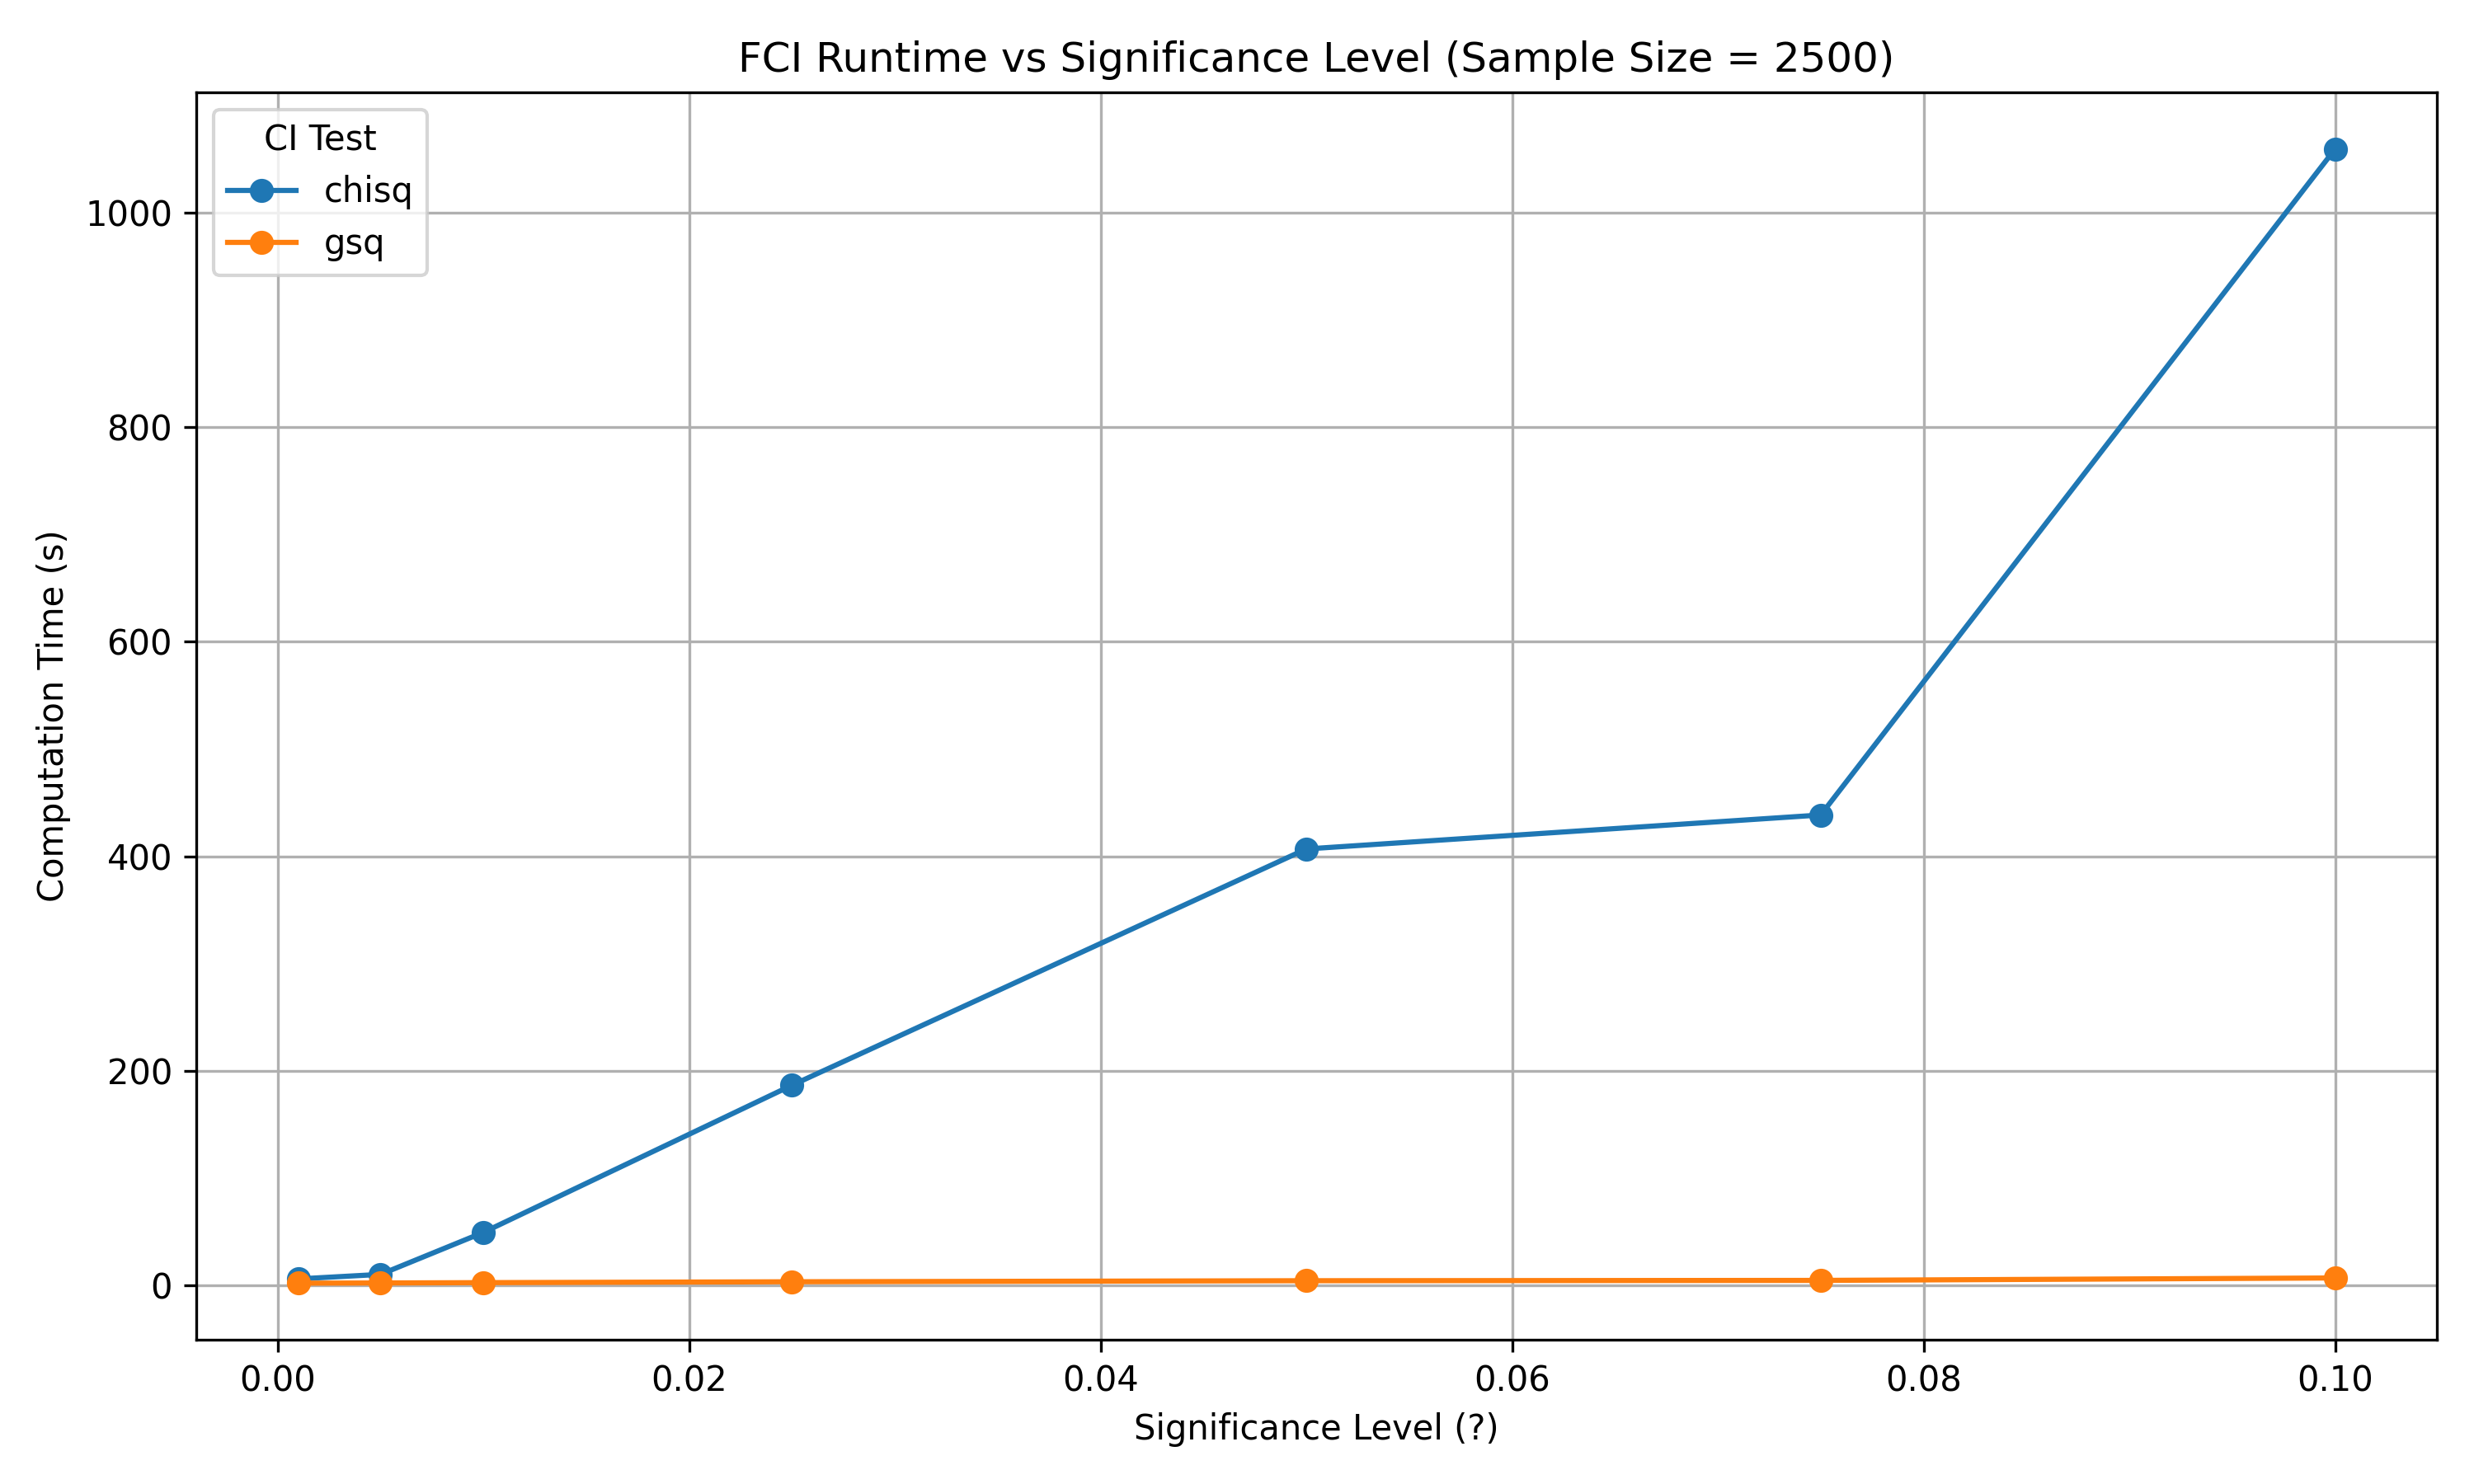
\includegraphics[width = 1\linewidth]{Report/final_report/pictures/fci_runtime_vs_alpha.png}
        \caption{Computation time of the FCI algorithm across different significance levels $\alpha$ for various conditional independence (CI) tests. Results are based on a fixed sample size of 2500 observations.}
        \label{fig:fci_runtime_vs_alpha}
    \end{minipage}
\end{figure}

During the experiments, we ran through $\alpha$ = [0.001, 0.01, 0.05, 0.1]. We also test how differently $\chi^2$ and $G^2$ will perform given $\alpha = 0.01$ on 6660 samples. 

% \subsection{Software and Implementation}
% In this report, we used the causal-learn library for Python to perform causal discovery on observational data. 


\end{document}
